\documentclass{l4proj}
\usepackage{url}
\usepackage{indentfirst}
\usepackage{graphicx}
\usepackage{wrapfig}
\usepackage{caption}
\usepackage{float}
\usepackage{listings}
\usepackage{courier}
\usepackage[svgnames]{xcolor}
\usepackage[colorlinks=true,
			linkcolor=DarkRed,
            urlcolor=Navy,
            citecolor=DarkGreen]{hyperref}

\begin{document}
\title{Level 4 Project Report - A Large Scale Pedometer Application}
\author{David Mcinnes\\ \\0901288m@student.gla.ac.uk}
\date{28th March 2014}
\maketitle

\begin{abstract}

This report describes Hotsteps - an application with a number of aspects - a pedometer application, a website and associated backend software. The user places the app running on their phones and leave it running over the course of the day. It tracks the number of steps they make each day as well as the locations that those steps occur in. This information is then synced with a database located on a central server. A supplementary website uses this information to provide information to the user, such as Leaderboards, personal step counts and Heatmaps showing the areas with the most user activity. The application and website are designed to motivate users into using the application to track data and motivate their walking activity, and also to create a byproduct, that by-product being the data about steps totals and times, and the location/heatmap data. The app implemented was a good start in developing such a system, but would require additional and more fun features, such as groups of friends, improved battery life and mitigation  of the privacy concerns conveyed by the users during the evaluation. Once this has been completed, a larger scale evaluation and further research into the applications of the data logged could be carried out.

\end{abstract}

\renewcommand{\abstract}{Acknowledgments}
\begin{abstract}

I'd like to thank my supervisors, Dr. Alistair Morrison and Dr. Matthew Chalmers and everyone who helped me when I was stuck, and took part in my evaluation.

David McInnes

\end{abstract}

\educationalconsent
\tableofcontents
%==============================================================================
\chapter{Introduction}
\pagenumbering{arabic}

The aim of this project was to produce and implement a large scale pedometer app using phones and the Internet in order to provide a large scale infrastructure for pedometer usage. This is interesting because fitness and wearable technology is going to be an ever increasing area of importance in technology and Human Computer Interface. The near ubiquity of Gyroscopes and Accelerometers in devices such as modern smartphones and tablets mean that this is more feasible than ever before. Additionally, some high end smart phones as of 2014 have included 'Coprocessors' in order to provide a specialised processor to facilitate the tracking of such user activity. The iPhone 5S has this ability, as well as some Android smartphones. 

The premise of the application was such that users would prefer to not have to carry around separate devices in order to track their walking activity - it would be good if one device that eveyone carries around regardless was used. In today's world, most people carry around mobile phones, with most of these being smartphones in 2014. This means that the modern mobile phone with its near ubiquty and in-built Accelerometer and Gyroscope is the perfect candidate for this. Instead of a seperate device, just use the mobile that most people have in their pocket. The application acts as an app with a by-product, that by-product 

\section{Background}

A current area of intense research and interest in the field of Human Computer Interaction is wearable technology. Items that purportedly increase the users likelihood of carrying out exercise are increasing in popularity. Many applications, features and products have been introduced in the past couple of years such as Endomondo that are designed to gather information about the users physical, displaying this as information useful to the user as 'Quantified Self' technology. 

Wearable technology and technology that is designed to increase the users health levels is going to be an increasingly important part of technology as time goes on - it is possible that software such as this could be of a massive benefit to health in general.

With this in mind, there are different ways to provide a niche for a new Pedometer application. It would be interesting if there was a communal way of tracking all of the users of an application communally, with communal information about usage statistics amongst all of the applications users. This could be useful in a whole variety of contexts. If users liked it as a method of promoting regular walking activity, then it could be further expanded to support this usage. Additionally, the location and step tracking throughout the day provides a number of possible benefits to numerous companies or public bodies that might be interested in seeing where users walk throughout the day, and how much walking people are doing. For example, prospective businesses may be interested in viewing what areas are popular with walkers at what time, on order to get an idea of where might be an appropriate place to start a business.

In the next year or so, the prevalence of such devices will increase massively in everyday usage, meaning that there is likely to be an increase in demand for apps such as Pedometers and fitness trackers. 

\section{Project Outline}

The goal of this project was to create a pedometer for Android based phones that runs in the background over the user's day, logging useful data about the number of steps the user is making every hour, and also track the coordinate location of those steps. When the user leaves the house in the morning, they turn the application on, and they simply leave it running whilst they go about their daily business. When running in the background, the application tracks the number of steps the user is making and uploads them to a central server hosted by the department every ten minutes. In addition to tracking the number of steps, the application also regularly captures the location of the user as they walk around. These locations are stored until it is time to sync with the server. In conjunction with the application, a website was also implemented that complements the application. Users can use the same login information from the application in order to access their information on the website. This website contains aggregated information amongst all of the users of the application, as well as their own information. Users can view Heatmaps that use the location information uploaded from the app. These heatmaps display the most popular areas that users frequent. The standard Heatmap created are that of aggregated data for all of the users, and your own information per day. Users can also create personalised heatmaps between any new time frames.

The reason that this app was implemented was as a way of getting data about number of steps made per day during 15 minute intervals, and the locations of those steps to be displayed in a Heatmap. The goal of this project is not to propose a specific use for this data, though some ideas will be described, but also to implement a system that promotes the usage of the application in order to harvest this data from users. By adding data tracking features like leaderboards, steps by day, aggregate all-user data and Heatmaps it was hoped that the user would enjoy this enough for it to be a worthwhile system to harvest this data, followed up by an evaluation to find out what users liked, disliked, and felt concerned about. 

Battery Life
Is it interesting enough?
Privacy concerns?

\section{Document Outline}

The Literature Review takes a look at previous similar research and applications in the field of applications with by-products, so called 'motivated-self' applications, and previous work in the field of activity/location tracking, and how this previous work relates to the themes examined in this project. In addition, the issues of privacy in large scale systems that track user location data are also discussed.

The Requirements chapter describes all of the functionality, functional requirements and non functional requirements that that it was necessary to be integrated into the Android application and website.

The Design chapter goes through the choices of features used in the project, and why those features were chosen. Additionally, the rationale behind the User Interface design and wireframes showing the idealised design of the application are discussed.

The Implementation chapter goes through the code internals and gives an overview as to what progamming languages and technologies were used, what limitations the current version of the system has and the reasoning behind the choice of certain technologies or rejection of others.

The Testing chapter shows the testing to confirm the success of the app in areas such as the accuracy of step counts, the accuracy of results on the website, and issues that occur on some phones or browsers but not others. 

The Evaluation chapter describes the user evaluation that took place in order to determine the success ot lack thereof in two key areas:

\begin{enumerate}

\item{Is the app interesting enough? Does it do enough to motivate users to use the app and provide data, and are the 'quantified self' features strong enough to facilitate user motivation to use Hotsteps?}

\item{Are there privacy concerns from users about their location data being tracked whilst using the Hotsteps system? Are these concerns enough to put users off of using the application? Is there anything that can be done to mitigate and minimise these concerns.}

\end{enumerate}


%==============================================================================

\chapter{Literature Review}

Before undertaking the project it was necessary to undertake a review of recent literature from similar topics and products.

There were a variety of research papers that informed my approach to designing and implementing the system and designing/carrying out the evaluation upon the system. In this section, each of these papers will be discussed and how their findings relate to the system.

\section{Games with by-products}

\subsection{The ``ESP" game}

Given the focus on getting users to use the application in order to produce a by-product (the step and location data), a seminal 2004 paper on an interactive system (in this case a game called "ESP") that simultaneously is enjoyed by the user and gives a valuable by-product is 'Labeling images with a computer game' by Von Ahn and Dabbish [1]. The paper describes a game whereby the user is presented with photos and enters 'keywords' for that image, whilst getting a simultaneous user to "agree" on a keyword. Say for example the users are presented with a picture of a brown purse. Words that might come to mind are "purse", "bag" and "brown", which is entered by the first user. The first guess typed in by the second user is "handbag", which doesn't match any of the input keywords by the other user. The second user then inputs "purse", which does create a keyword match between the two users. In reward for matching each other, both of the users are rewarded with a certain number of points. If they can agree on fifteen images, then both users get a large number of bonus points. Users are promoted to continue using the application by the presence of a "thermometer" on screen that continually fills the closer the users get the completion. The game is made more complex by the presence of up to six "Taboo words" - words which have already been agreed upon many times for that image and hence are not allowed to be used again. This increases the richness and number of the labels for each image in the game.

The hugely beneficial by-product from the ESP game is that of labelling and categorising images on the internet, ideally those images indexed by search engines. Doing so would improve image search reults massively. Traditional techniques such as computer vision and analysis of the text nearby images had not been successful, but using the human mind was considered perfect for this task. When the two users agreed on a image description, this was typicaly a good label for that image. A major aspect of the evaluation of the ESP game isthat the users are never asked to enter keywords describing the image on screen, but that evaluation of and usage of the game has shown that users do in fact enter accurate labels for the images in the game. Data showed that the game could be agreed upon as being fun - users sent a lot of time playing - 50 hours in some cases! - and most people played at least once. 1.3 million labels were created with only 14,000 users, with the assumption from that being users enjoyed the game. The game was very successful at acheiving high quality by products, the descriptions of images were accurate and helped image labelling, and at the rate of use at the time of the evaluation, could have indexed all of the images on Google images within weeks. As the authors concluded, what would normally be considered tedious work had been transformed into "something fun to do".

\subsection{Eye-Spy}

Another paper that builds on the "ESP" game describing a game with a by-product is "Eyespy: Supporting Navigation through Play", a 2009 paper by Bell et al [2]. The paper describes "Eye-spy", a game designed to extract picture and location data from users. Whilst using the app, players 'tag' geographic locations with pictures or text, and when other users visit that tag, they can "confirm" them, gaining points for doing so, and also verifying the accuracy of the tagging. Eye-Spy was judged to be successful, not only as a game (users commented that using the app gave them great enjoyment in visiting areas they had visted many times before, allowing them to view locations in a new light), but also in creating useful augmentations of maps with the accuracy of crowd confirmed correctness of images.

\subsection{Crowdsourcing}

Both the ESP game and Eye-Spy use the concept of 'crowdsourcing' in order to create and extract data about images or the environment.  Crowdsourcing is a technique with growing popularity and usefulness in the field of data gathering 

\section{Motivating User Usage}

Obviously in order for users to get the data they must be at least semi motovated to putting their time and effort to use the app. A growing category using technology in recent years is that of the 'Quantified Self', described by Bell as "the regular collection of any data that can be measured about the self such as biological, physical, behavioural or environmental information'. This tracking could include logging of the users diet for weight loss and diet purposes, as well as activity tracking, whether that be running or walking, or other forms of exercise. Examples of such devices on the market include the FitBit and Nike Fuelband, which track exercise sessions and totals of their users.

In the 2009 paper "Emerging patient-driven health care models: an examination of health social networks, consumer personalized medicine and quantified self-tracking", Swan argues that there is a whole new category of patient-driven medicine services, including so-called 'Quantified-self' tracking [3]. The paper makes that point that the prevalence and availabilty of such technology has been limited in the past due to high cost and lack of tools, but improving technology and the prevalence of such technology has placed this category of application into the hands of end users, be they websites or services, or wearable devices such as the FitBit. All of these devices ostensibly provide a benefit to the user - they keep track of the exercise and activity of the user, or track the number of calories they eat each day, taking some responsibility away from the user and make the data logging as seamless as possible. 

Rooksby et al. descibe the use of such activity trackers as "lived informatics" in the paper "Personal Tracking as Lived Informatics" [4]. It provides an overview of the different types of personal trackers available, and extensive anecdotes from users of devices such as FitBit and applications such as Endomondo. There were a number of interesting findings in the area of social tracking, notably that users tend not to be particularly impressed with integration to social networks such as Facebook and Twitter, as is traditional amongst apps in the activity tracking category. One user mused that standard actions such as a user posting about the length of their run on Facebook as "kind of egotistical ... it’s almost one of those things where you set yourself up for failure". Standard social functionalities such as befriending were less engaged with than more anonymous social features, and  The paper proposes greater focus be more mindful of simultaneous tracking, friendship, competition and play.

\section{Previous Systems}

\subsection{Ubifit Garden}

UbiFit garden was an early smartphone application that aimed to provide a stimulus to increase user activity of the mobile phones. Given the era that this application was develeoped in, the application requires additional hardware bolted onto the back of the phone. Given modern conveniences, many people would consider this to be an unacceptable drawback to the application, but for a time when smartphones did not have included accelerometers and gyroscopes to be able to internally handle such applications.

Ubifit Garden was designed to be used by the user throughout their day to day business 

\subsection{Shakra}

Shakra was a research paper published in 200

\subsection{Houston}

This was a research paper published in 2006 

\subsection{Nintendo 3DS Pedometer}

There are a number of products on the market that act as a pedometer for users to keep track of their steps. An example of this is the 'Activity Log' application in Nintendo's 3DS Handheld video game system. Whilst the system is on standby in the users pocket whilst they walk around, it tracks the number of steps they are making throughout the day. Ostensibly designed to promote user activity through walking, the application contains a number of elements of note. Users are motivated into using the application by being given more play coins the more steps they make each day, up to a total of ten. These play coins can be used to buy items to make progress in games, or receive unlockable content. This provides additional enjoyment to the user, and by carrying out that task, the user receives a benefit to them. The activity log also contains a by-product with a benefit on Nintendo's part, as by the act of having the user walk around with the system in their pocket, Nintendo gains valuable data through the 'Street Pass' application in addition to motivating users to carry around their video game system all of the time, and at the same time providing benefits to users.

\subsection{Endomondo}

Endomondo is an application for iOS and Android that tracks the users sporting activity sessions, whilst using a device with an established GPS connection. The app tracks the type of activity being carried out by the user (say, Running) and logs information about the duration of the activity, the distance covered, and the number of calories burned. Users can also view augmented maps showing the location data of their activity, for example the route that the run took place over established by GPS. Users are motivated to use the app through these Quantified Self features, and by using the application they are getting valuable data about themselves that without having to manually record all of this data themselves.

\section{Privacy}

With applications and systems that track user locations, privacy issues are a growing and ever more relevant concern when developing large scale applications. A number of research papers have looked at this topic and how to mitigate user concerns around privacy issues. Krumm summarised that studies "show that people are generally not concerned about location privacy, although they are sensitive to how their location data could be used, and their sensitivity may rise with their awareness of privacy leaks".

%==============================================================================

\chapter{Requirements}

\section{Proposed System}

Taking into account previous examples of and research in the field, a system called Hotsteps is proposed that consists of an Android application and associated website for viewing data stored on the system's database. Users will install the app and create an account, and on log-in will instantly track the number of steps that user is making not only on a daily basis but also the number of steps every 15 minutes. Similarly to Endomondo and the 3DS Activity Tracker, the app will aim to motivate use of the app amongst users by giving them activity logging and motivated self functionality that is interesting and hopefully fun. Users will be able to view aggregate data from all of the users about step totals for all users from that day, a chart showing what hours of that day had the most steps from users, and a Heatmap that aggregates all of the location data for that day. The busiest areas of activity will have a deep red colour to signify high activity, middling areas with yellow, and areas of low activity coloured green. Areas with no activity appear as normal. Building on the findings of Rooksby et al. [3], the social integration proposed in the application is focused upon competition through the leaderboard functiionality and collaboration in order to endure the community increases its step count everyday.

It is not intended that the application is used to promote fitness and activity amongst users per se, as some of the examples in the Literature are designed to do. Arguing such a hypothesis would require a far more lengthy and in-depth user evaluation carried out to verify those claims. Despite this, given the applications status as a Pedometer with hooks to motivate the user to continue using it, and that users were unlikely to be put off walking more by using Hotsteps, any theoretical increase of motivation to walk would still be a good thing for individuals health, and, importantly, would ensure that the user continued to provide data for the application, the importance of which is explained below.

In addition to the front-facing user enjoyable aspects, Hotsteps is also intended to be an application with a by-product, in that the data logged by many users walking around and logging their steps and locations is theoretically valuable to a whole range of organisations and use-cases, such as urban-planning, health-planning, entrepreneurs or even tourists. The use of the Heatmaps is an interesting by-product in that it is intended that the app users themselves will also enjoy the heatmap functionality as part of the 'Quantified Self' features, 

\section{Non-functional Requirements}

\subsection{Operation at a large-scale}

Given the large scale features of the proposed application, the system must be able to work on a scale such thaat many simultaneous users  wil be logging and receiving their data between the app and website. It is not envisaged that the system will be particularly widely used my thousands of people at the same in the scope of this project but it must be able to handle multiple users at the same time without losing any data or taking an excessive time to sync with or pull from the server. 

\subsection{Security}

User data must be secure and behind a login wall such that only a user will be able to see their personal data.

In order for a user to use the Hotsteps system, they must create an account. Having to create an account solves two problems. User data such as step total and location data can be stored as part of the users account, and users can be sure that their information would be associated with their account.

Additionally, the account system must be secure, with 

\section{Functional Requirements}

\subsection{Android Application}

In order to be able to track the users steps, it was necessary to implement a Smartphone application that would be running whilst the user had theur smartphone in their pocket. The app must work in the background whilst running in the users pocket. It should be relatively conservative on users battery life, and also must be able to track the users current location whilst using the app on a regular basis. There must be a log in screen that allows users to enter their username and password to enter the app and associate their usage of the app with their own account. Additionally, there must be the functionality for users who do not have an account on the service to be able to create one. Once the user has been logged in, the application should start tracking the number of steps they are making and be able to display this to the user in a visually obvious manner. Additionally, it should provide the ability to manually sync with the server and provide a visual indication of daily leaderboards and how many steps the user has made on previous days, though it is intended that the majority of the data viewing capabilities will be reserved for the website due to a limitation in development time and the ease of website development compared to Android applications.

\subsection{PHP Backend}

It was necessary to implement a backend server to provide the data services for the Smartphone application. This will receive the data sent over the network from the application and handle it in the appropriate manner. When an HTTP POST request is sent via the app to update the server about a users step total or location data, then these scripts handle the data sent using the requested script. This could be adding data to the database, querying the database to display information on the website or application, or carrying out user authentication and cookies for the website.

\subsection{Database}

It was necessary to design and implement a database to store the data required for the application and website. This database should store user accounts, assign them a userID, and store all of the steps by day and by hours of that day. The database should also store the list of user locations indexed via date and time in order to provide coordinates  for the heatmap data. The data would be added and queried to using the PHP back-end and this will provide and receive data to the app and website.

\subsection{Website}

In order for the user to have a way to access the information, it would be necessary to design and implement a website that will allow users to view their step totals for days, and also to display Heatmaps that make use of the location data that is harvested by the app.

%==============================================================================

\chapter{Design}

The rationale behind the design of the Database, App, backend and Website is explained.
\subsection{Database Design}

When beginning to consider storing the user data, it was necessary to design a Database that would effectively hold all of the necessary data, be able to query that data in a reasonable timeframe given the mobile nature of the project.

\begin{figure}[ht!]
\centering
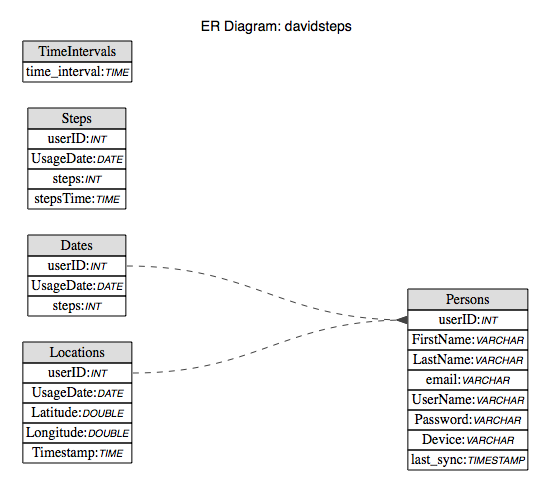
\includegraphics[scale=0.5]{images/screenshots/erdiagram.png}
\caption{\textbf{Displays the Entity Relation diagram for the Database designed}}
\label{design:erdiagram}
\end{figure}

A diagrammatical representation of the design of the Database is seen in Figure \ref{design:erdiagram} in the form of an ER (Entity-Relationship) diagram.

\subsubsection{Users Table}

\begin{figure}[ht!]
\centering
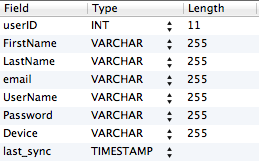
\includegraphics[scale=1.0]{images/screenshots/usersscreen.png}
\caption{\textbf{Displays the attributes of the Users table of the Database, as well as their type.}}
\label{design:usersscreen}
\end{figure}

The table Users stores all of the data about the usernames of the app. userID, Firstname, Surname, Email, Username, Password (stored as an SHA-256 Hash), and a Timestamp signifying the last time the user pinged to the service, so it can be seen if people are using the application. The attributes and types of this table can be seen in Figure \ref{design:usersscreen}

\subsubsection{Locations Table}

\begin{figure}[ht!]
\centering
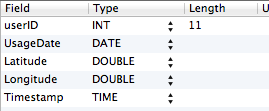
\includegraphics[scale=1.0]{images/screenshots/locationsscreen.png}
\caption{\textbf{Displays the attributes of the Locations table of the Database, as well as their type.}}
\label{design:locationsscreen}
\end{figure}

The next Table is Locations, which stores all of the Latitude and Longitude pairs uploaded to the service. The attributes and types of this table can be seen in Figure \ref{design:locationsscreen}

Each location is associated with a userID, to make it known what user was in this location. This is integral for the website aspect of the Project. Each Latitude and Longitude originates from a user of the application whilst using the application. These are stored as doubles due to the floating point nature of precise coordinates.

\subsubsection{Steps Table}

\begin{figure}[ht!]
\centering
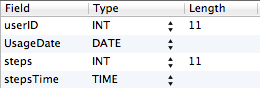
\includegraphics[scale=1.0]{images/screenshots/stepsscreen.png}
\caption{\textbf{Displays the attributes of the Steps table of the Database, as well as their type.}}
\label{design:stepsscreen}
\end{figure}

The final table in the Database is the Steps table, which stores the amount of steps each user has made in a 15 minute interval. Whenever the user uses the service for the first time each day, a record is added in the Dates table for each 15 minute interval in that day. A limitation of this is that a number of records each day will essentially be empty and have 0 steps, taking up storage space for the database. The trade-off was to either make the data harder to traverse and re-assemble when it comes to using that information in the application or website, or save space and make re-assembling the data somewhat harder. Having gone over the different options, the former option was chosen, though there is no technical reason why this cannot be changed in the future if space was becoming an issue. Whenever the app refreshes its sync with the server it checks what 15 minute interval the set of steps occurred in, and add the number of steps that occurred in that set of steps to the total for that 15 minute interval. The attributes and types of this table can be seen in Figure \ref{design:stepsscreen}

\section{Application Design}

For the design of the Android app, consideration was made as to what UI elements should be front and centre of the users view at any given opportunity and started to make some prototypes based upon that. A wireframe showing the initial application design at the Design stage is shown in Figure \ref{design:appwireframe}.

The top bar of the app shows the name of the screen the user is currently viewing, and well as a menu for the user to navigate around the app - options in the menu will include functions such as Settings ang Log Out.

\begin{figure}[H]
\centering
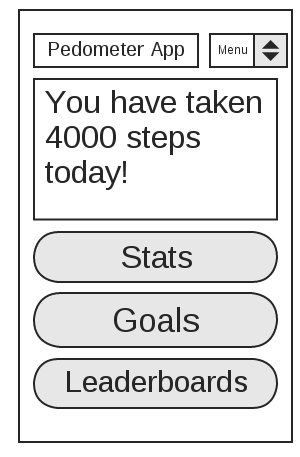
\includegraphics[scale=0.7]{images/diagrams/appwireframe.png}
\caption{\textbf{Wireframe of the User Interface of the Android application during the design stage. The step totals can be seen, as well as the menu dropdown, and options for statistics, goals and leaderboards. Goals was left unimplemented in the final application.}}
\label{design:appwireframe}
\end{figure}

\subsection{Step Count View}

As seen in \ref{design:appwireframe}, the main UI element of the main screen of the app to be the number of steps the user has made that day. This view was designed to be eye-catching and instantly grab the attention of the user to their step count.

\begin{figure}[ht!]
\centering
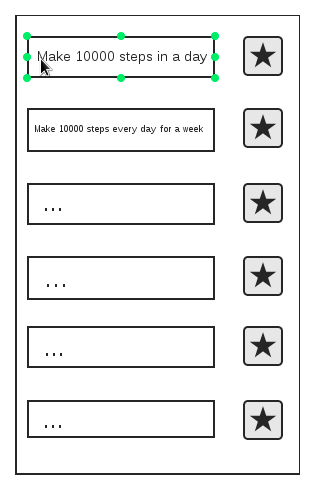
\includegraphics[scale=0.7]{images/diagrams/goalswireframe.png}
\caption{\textbf{Wireframe of the User Interface of the Android application during the design stage. The proposed Goals screen can be seen, including some examples of Goals to be completed by the user. If the user had completed the task, then the star would appear filled in.}}
\label{design:goalswireframe}
\end{figure}

Below the sentence displaying the days step count for that user are buttons to navigate to the other sections of the application, such as the statistics and leaderboards views. There had been plans to include a button to proposed Goals functionality, that would include a number of goals for the user to complete. These could take the form of 'achievements', an example of an achievement that could be implemented could be "Achieve 10,000 steps everyday for 7 days straight". If the user completed an achievement, they would be rewarded with medals, which can be of different colours (Bronze, Silver and Gold), depending on the difficulty of the challenge completed. A wireframe showing the proposed design for this feature can be seen in Figure \ref{design:goalswireframe}.

There are a number of issues that may need to be addressed before the goals and achievements feature could be successfully implemented. These goals are designed in order to provide motivation for the user to walk and to use the app. Therefore it might be expected higher level goals would be somewhat harder to achieve. It will be necessary to receive guidelines on what kind of activities would be too excessive and potentially harmful for the user, in differentiation from goals that might provide a legitimate challenge but is still safe and fun for the user to attempt.  Considering such risks would involve discussion with medical staff or medical researchers.

\subsection{Statistics}

This screen of the app shows all of the previous days step totals from that user. Viewing all of the previous step totals is a useful feature for the user since it gives them an idea of the amount of steps they are making over time and whether they are keeping up with or falling behind in maintaining a high level of activity day to day. Additionally, it is hoped that this feature will promote and motivate the user into making more steps to match up to and beat the previous days in which they used the Hotsteps application.

\subsection{Leaderboards}

The leaderboards screen shows all of the users of the app's step totals for the given day, in descending order. Similar to the other features built-in to the Hotsteps application, Leaderboards is a feature designed to promote continued use of the application by users by getting users to compete against one another for not only the highest number of steps (and hence additional step and location data!) for that day, but also that week and that month, giving players a number of angles to compete with other users through the leaderboards.

\section{Website Design}

There were a variety of different factors to be considered for the website aspect of the project. It was an absolute necessity from the beginning of the development process that the account system would be common - users must be able to Log In to both the website and the Android application using the same account.

It was also wanted for the website to be modern and eye-catching, with up-to-date web technologies used throughout.

\subsection{Heatmaps}

Given that there would be heatmaps embedded in the website, it was necessary to think of designs for heatmaps and what might be considered necessary in the design of these. Commonly, heatmaps use a colour scale from green to represent light data coverage, to amber for moderate data coverage, and finally red to represent areas of the highest data concentration. These colours may be standard and appropriate for most users, but some people are likely to have colour blindness and therefore make it difficult to distinguish between or understand the colours represented. Therefore, when choosing a library or toolkit to provide these heatmaps in the finished website, it would be necessary for it to provide an option for colour blindness, as well as the possibility of increasing the radius of each data point on the map, to help people who may not be able to pick out or see the data points as effectively as intended. 

Addtitionally, if there is a lot of data in the heatmap, then there should be the functionality to increase the radius of the data points on the heatmap, thereby making them appear much bigger. This has the benefit of making the data look much more obvious if there is little data for that day. 

%==============================================================================

\chapter{Implementation}

In order to successfully implement all of the software required for the project, there were a number of new programming languages and concepts to become comfortable in using. For example, I had no knowledge of PHP but had to learn in order to implement the back end for my project. I followed some tutorials to quickly learn PHP in order to have enough skill to be able to implement what I need to. I carried out development using the Eclipse IDE, the de-facto standard for Android development currently, though alternate IDEs are in development with the mind of replacing the Eclipse IDE as the recommended choice, such as Android Studio.

A diagram of the system overview as implemented can be seen in Figure \ref{impl:dia1}. As can be seen, the system consists of two different types of client. Firstly, the app user, who interacts with the server to download their current step information when logging into the app, as well as some basic statistics for view in the application. The second client type, that of the website, interacts with the server back end to query information such as step totals, leaderboard information and coordinates to display on the website heatmaps.

\begin{figure}[h!]
\centering
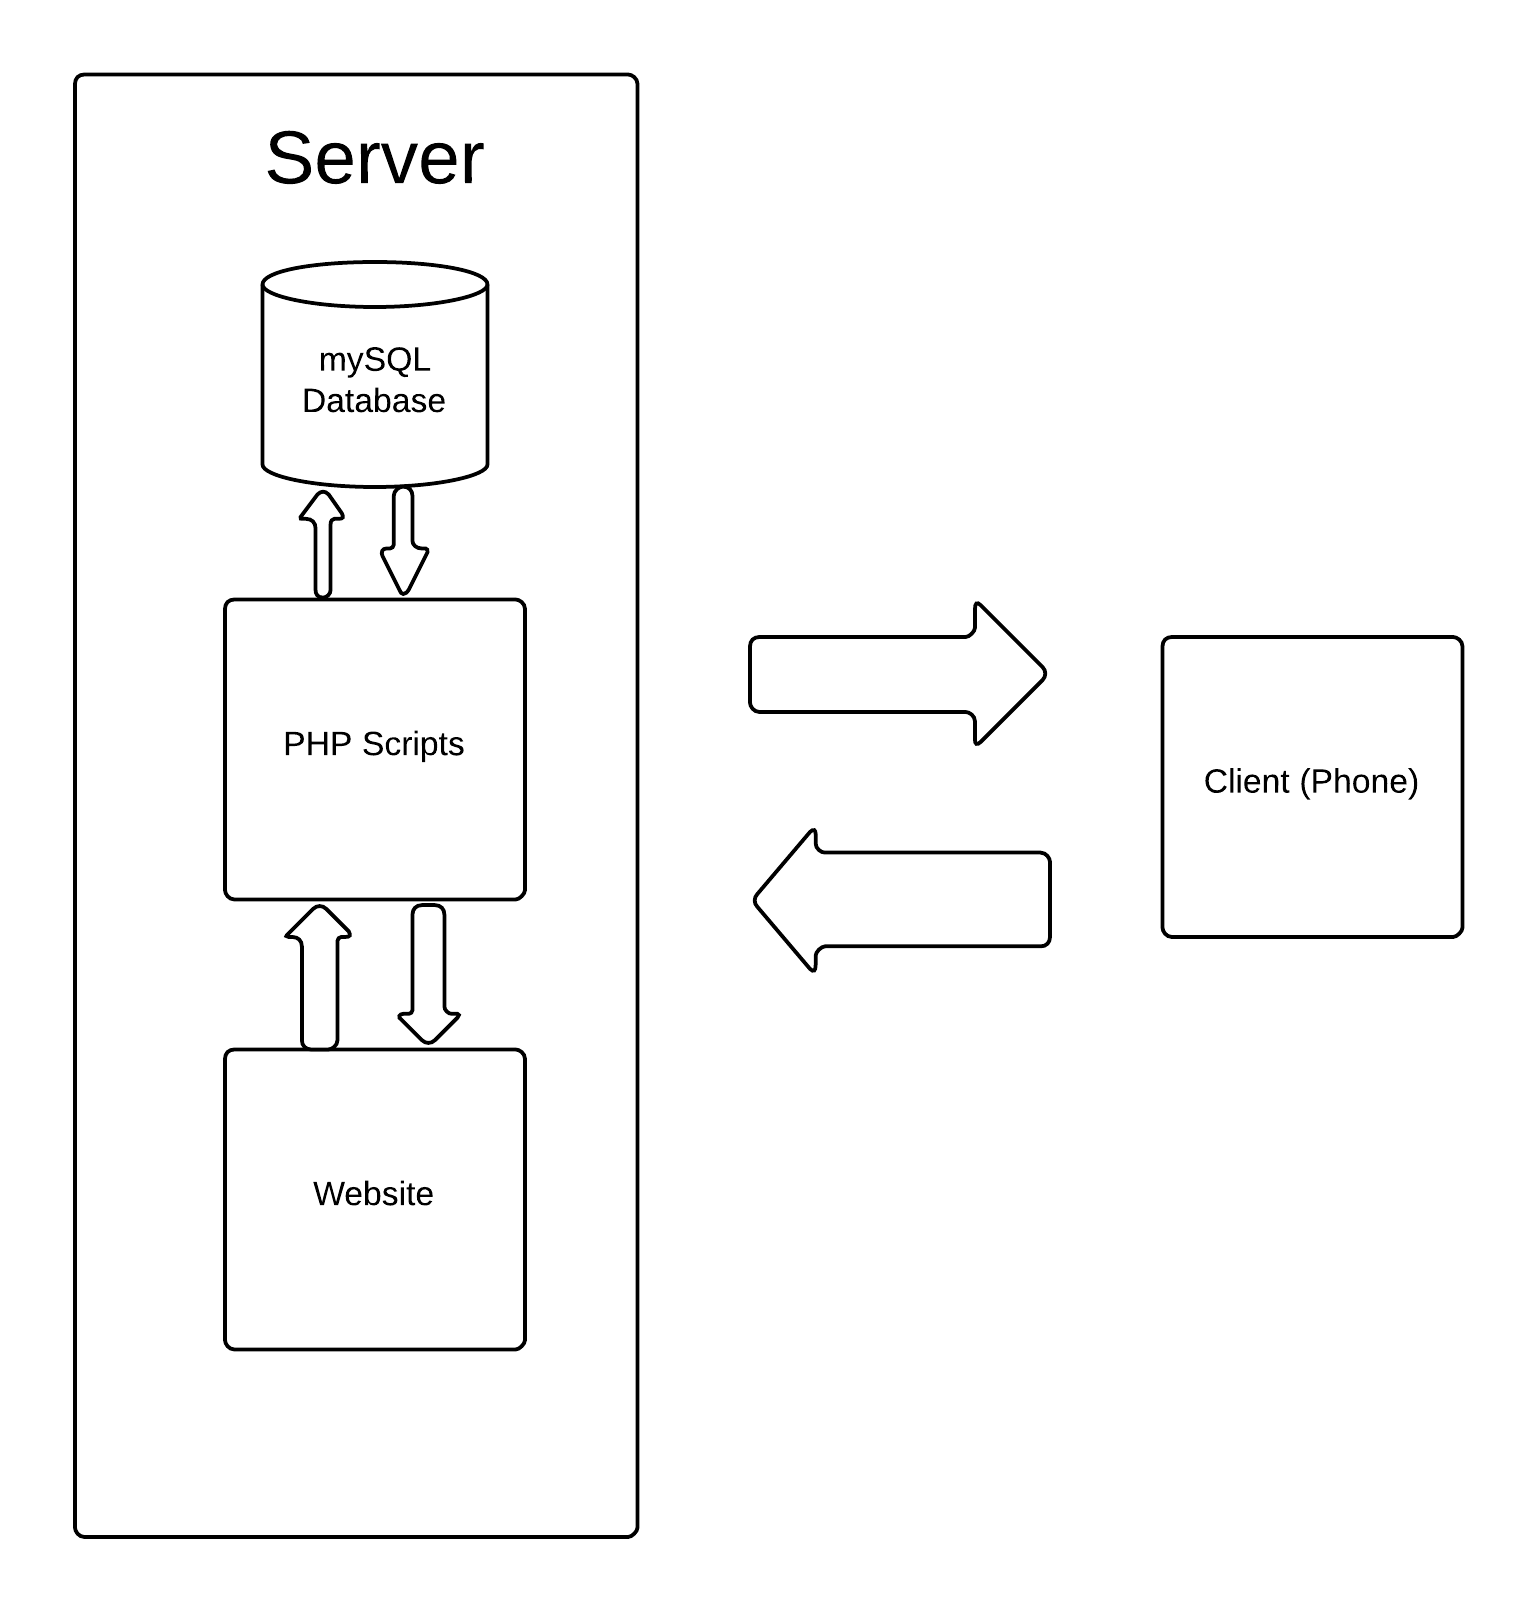
\includegraphics[scale=0.1]{images/diagrams/systemoverview.png}
\caption{\textbf{Diagram of the System Overview. The server which hosts the Website, PHP scripts and Database communicates back and forth with the phone and website acting as the Client.}}
\label{impl:dia1}
\end{figure}

\section{Android Application}

In this section, the implementation of the Android application aspect of the project is described, why specific technology decisions were made, and other technical aspects relating to the implementation.

\section{Technology Choices}

\subsection{Choice of Mobile Operating System}

Before development began, it was necessary to decide what technology and OS the app would be implemented in. Given the popularity of iOS and Android in modern mobile phones, I decided to choose between these two. Development in iOS uses the Objective C language, which is predominantly used by Apple. A lack of experience in using the Objective C language was also a barrier. Additionally, iOS development requires the use of the XCode IDE, which is only available on Mac OS X.  While it was easy to get access to the software, development would be slightly more logistically challenging given that it was likely that development would take place on a number of different machines. On the other hand howver, with iOS there would be a far smaller number of possible devices that the app would have to be designed to support. One of the major obstacles involed with choosing Android development over iOS is that there are a much greater number of devices that use Android at any given time versus devices that use iOS. Whilst iOS devices are generally all within the high end range of current technology, Android devices can vary wildly in CPU speed, internal memory, and screen resolution. This means making a possibly complex decision about which type of devices to target development for.

Android development is cross-platform on the Linux, OS X and Windows Operating Systems, meaning any computer could be used for development purposed. This would make development logistically easier. Additionally, Android development uses the Java programming language, with which there was a greater personal affinity to and also experience of writing code for, having done it in many courses and having used it as the implementation language for the Level 3 Project. 

Regardless of what system or OS was chosen, both are very well documented on the World Wide Web, with plenty of guides and tutorials available to explain both high level concepts and coding skills for those platforms.

Given the available choice outlined above and going through their pros and cons, it was decided to develop the system for Android OS due to previous experience with Java, making it less likely that development would reach a snag or be slower due to my inexperience with Objective C. In future, the app could be ported to iOS if usage of the app was shown to be popular or it was requested by user feedback and it was shown that more data could be logged on the system through such a development.

\subsection{Implementation Overview}

One of the major concerns throughout implementation of this project was to get the application to such a state whereby battery life is not excessively drained by  near constant usage of the application as it is designed in anticipation of. Modern smartphones generally have relatively poor battery life given their high processing power, high-resolution screens and regular network operations. These network operations can happen regularly, and if not managed in an efficient manner  they can cause a real negative impact towards the battery life of a device. If an application is causing the user's battery life to be at an unacceptable level reguarly, most users would simply rather delete the application than continue using it. Therefore, when making design decisions regarding the User Interace and network operations the main priority in determining the implemented behaviour was that of saving battery life.

The first stage of implementation involved getting to grips with Android development, which I had little experience in. This involved reading tutorials on the Android developers site, which has a good introduction to Android development that teaches me the basics, such as learning about Views and Activities, as well as show to travel between and move data between views using Intents. \textbf{\textit{Views}} are written in Extensible Markup Language (XML) and describe the look and feel of the User Interface. User Interface elements such as TextBoxes and Buttons and GridViews are introduced to the UI here. The behaviour behind the UI elements are implemented in \textbf{\textit{Activity}} files, which are implemented in the form of Java classes. Each Activity class consists of a number of methods that are automatically called - the activity cycle of the application.

The application consists of 7 Activity classes. In Android development, files describing the layout, look and feel of the User Interface are written using Extensible Markup Language (XML), which represents different views and UI components in a hierarchical structure. The functionality of the app itself is implemented using the Java programming language. Such a technique seperates the look and feel of the app from the actual functionality - following the principal of separation of concerns. Errors in the UI code doesn't cause errors within the Java code.

Due to the time and location based nature of the application, whenever the location as detected from Play Services changes another object is data is added to the Array consisting of the number of steps in that interval, the time, and the location in question,  and it is obvious as to what type of code is causing the issue when the application has errors and does not compile.

\subsection{Removal of "Goals" functionality}

During the development stage, which was carried out under a limited timescale it was realised that it would not be possible to implement the Goals app as originally intended and described in the design section. The reasons for this were that this would be the hardest app feature of those described to implement, and would have involved massively increasing the scope of the app itself, the database and back-end, and also the data viewing functionality on the website. Unfortunately with the timescale left for implementing and evaluating the system it would have been infeasable to complete this part of the system. The removal of the goals feature may have a negative impact on the motivation of users to use the app, this should be considered when carrying out the evaluation of the system. 

Removal of this feature at this stage also mitigated the need to consult expert opinion on the types of goals or achieveents that could could be dangerous or cause harm for a user that trues to complete them all. This move would therefore save more time to spend implementing other parts of the system..

\subsection{Google Play Services and Location Services}

Google Play Services is an API available for usage by developers that enables applications to be able to access many Google provided services. In the Hotsteps application, Google Play Services is used to provide and access the location data whilst the user is using the app. Google Play Services is only available on official Android phones, and not those that only support the Android Open-Source Project (AOSP). This is a minor limitation to the number of devices that could be used in this application.

Google Play Services offers a number of granularity settings for the collection of location data. Users can choose between high accuracy mode, battery-saving mode and GPS only mode. High accuracy mode collects location data from a variety of GPS, mobile networks and local wi-fi networks, Battery saving only collections data from mobile and wi-fi networks, and GPS only uses solely GPS data. It is recommended that users of Hotsteps use "High Accuracy" mode under standard use, since it provides fairly accurate location data whilst being relatively reasonable on battery life. In comparison with the Endomondo tracker, GPS is not required for the service and does not go to nor need to be that level of granularity.

\subsection{Network operations and \texttt{AsyncTasks}}

Android does not allow Network based operations to occur on the main UI thread. This is the Thread that runs as part of the activity lifecycle. In order to carry out Network operations, Android provides a wrapper for one time use threads that perform a task not related to the UI thread. ASyncTask takes in zero or more objects and uses them to complete a method and another method upon completion of that method. When it is time for the Application to sync with the server, the Array of packets is passed to the AsyncTask, which sends this JSON data to the server via a POST request, along with the userID. The PHP script which is invoked, \texttt{updatedb.php} loops through all of the data objects, and updates the total number of steps for the 15 minute interval signified by the time in the 'steps' table, and adds the location along with the time and the date that it occurred to the locations table. Theoretically, data can be lost using this system. If the request never makes it to its destination or it is corrupt there is no error fixing, no resending, and the data once sent is not recoverable. This was considered an acceptable risk, as none of the data is critical and the odd loss on occasion is acceptable.

\subsection{\texttt{AccountLogin.java}}

When the app is initially loaded without a saved login, the first screen that loads is a Login.java. The User Interface for this view can be seen in Figure X.X. This consists of a standard user login screen, with TextFields for Username and Password. The field for password is a special UI element that covers up the characters entered. If the user does not have an account, they can move to the screen that enables them to create their own account using the 'Create Account' button. Once the user has entered their login details, the system checks using a POST request and response that sends the information to check whether or not the account exists in the database and whether the password corresponds to the one on record. If the login details are not correct, the user is informed through the use of a 'Toast' UI element, which displays a small message that overlays the rest of the screen. Once correct user credentials are confirmed, an Intent is sent to send the user to the main Pedometer screen of the application. 

\subsection{\texttt{AccountCreation.java}}

If in the previous screen has sent app execution to the 'Create Account' page, Before this appears, there is an information page that appears about the Terms of Use of the application, which informs users that their location and number of steps will be tracked. If the user disagrees, a Toast appears that informs the user that as they have not agreed to the terms of service, they cannot create an account, and then execution is transferred back to the Login screen. If the user accepts, then they are passed onto the Account Creation form, a screenshot of which can be seen in Figure X.X. This screen consists of a form that prompts the user for the details required by the applicaion and Database for user accounts. 

\subsection{\texttt{PedometerActivity.java}}

The main backbone of the application is that of \texttt{PedometerActivity.java}, which provides the code for the main view of the application. This is displayed after the user logs in. Once the screen appears, an object of type \texttt{StepCounter} is created that begins to track the users step count. This class displays the interface defined in \texttt{pedometeractivity.xml}, as seen in Figure \ref{impl:dia2}. There are a number of buttons the user can click on this screen. Hitting 'Statistics' will take the the user to a page that allows them to view all of their statistics, and 'Leaderboards' takes the user to a page that lets them see that day's leaderboards. 

\begin{figure}[ht!]
\centering
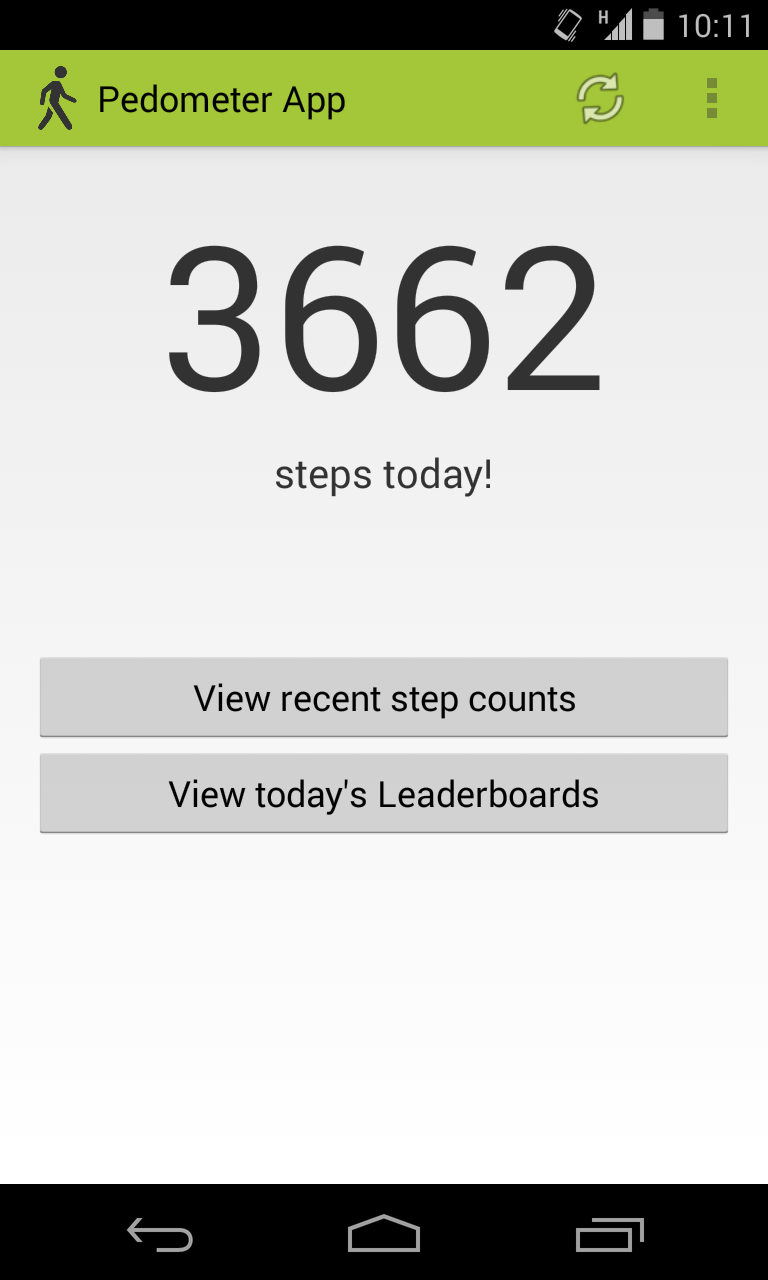
\includegraphics[scale=0.2]{images/screenshots/appscreen.png}
\caption{\textbf{Screenshot of the main view of the Android application, defined in pedometeractivity.xml and PedometerActivity.java. Note that the UI of this screen has changed since the original design wireframe to give a much greater prominence to the day's step total.}}
\label{impl:dia2}
\end{figure}

Whilst the app is running, whenever the location services integration detects a change in location, a callback method is called that stores the current time, the amount of steps since the last change in location, and the current Latitude and Longitude. This information is then encoded as a \texttt{JsonObject} and this object is stored in a \texttt{JsonArray}. 

In the background, the application is tracking the number of steps being made by the user. There is a localSteps count that displays the number of steps i There are a number of different aspects to the updating of the server with this information. There are two threads on a timer that are running alongside the app. The first of these updates the User Interface with the day's step total as you are walking around. The second of these sends all of the data packets (Stored as JSON) in the data array up to the server to be added to the Database every ten minutes. There is also a manual refresh button next to the menu drop down button in the top right corner, and when the app is set to background running it also performs a server sync.

\subsection{\texttt{SessionManager.java}}

It was necessary to provide a local data store on the device itself in order to save data that the user will not want to enter everytime, such as their login details. These are stored using Android's \texttt{SharedPreferences}, which saves data as Key-Value pairs locally on the device. In this scenario, if the user logs in and closes the app without intentely logging out, then their user data is saved and upon reopening the application, their profile logs in automatically. \texttt{SharedPreferences} also provides benefits for the internal transfer of data within the application. Instead of having to transfer pertinent information between views through the use of Android Intent calls, it could simply request the appropriate information through a call to the \texttt{SharedPreferences}. The main use for this in the application is to get the userID which is received from the database when the user logs in and is stored as a \texttt{SharedPreferences} Key-Value. Whenever one of the views in the app needs the userID of the current user, it makes a request to \texttt{SharedPreferences}, and receives the userID. In addition to being easier to implement and manage than Intent passing, this also reduced the possibility of user data becoming corrupted, as instead of being passed between views contantly, the values are set upon loading and simply called upon when needed.

\subsection{\texttt{StatisticsActivity.java}}

This class displays an interface consisting of a ListView defineed in statistics.xml. A ListView is a standard Android UI element that can be populated with content and which takes the form of a list that can be scrolled over by the user if it does not fully fit the screen of the device. When this class is loaded it sends a POST request to \texttt{jsonscript.php} containing the current userID as received from the central \texttt{SharedPreferences} store that returns all of the previous days Step Counts for that user as a list in JSON format. The JSON list is then parsed and added as elements to the \texttt{ListView} which are then displayed in the list.

\subsection{\texttt{LeaderboardActivity.java}}

\texttt{LeaderboardActivity} displays a \texttt{} as defined in \texttt{statistics.xml} to display the list of users who have used the app on the day in question and displays their step counts in descending order as a Leaderboard. This class sends a POST request to \texttt{leaderboards.php} hosted on Tethys which returns as JSON a list of users in descending order of Step Count for that day. The JSON is then parsed and the content extracted is reformed as readable text and added to the ListView and displayed. A screenshot of this screen can be seen in Figure 

\begin{figure}[ht!]
\centering
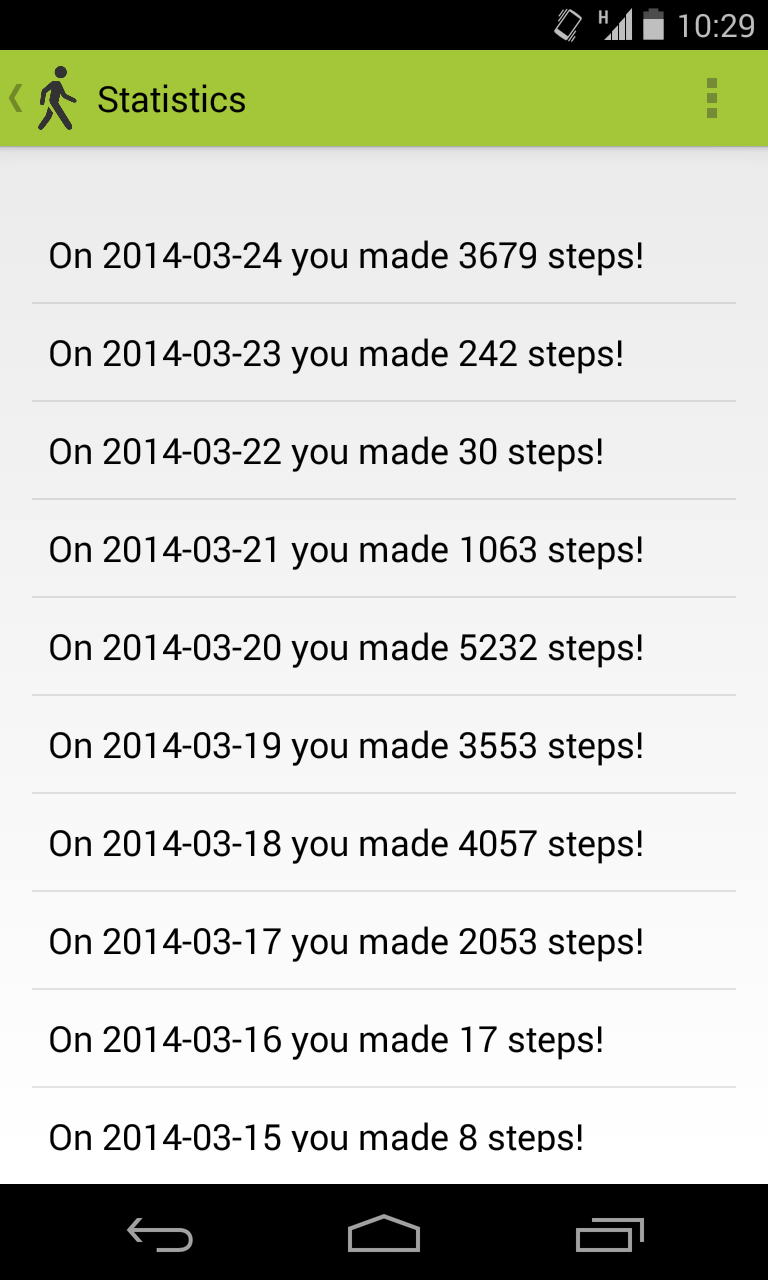
\includegraphics[scale=0.2]{images/screenshots/statisticsscreen.png}
\caption{\textbf{Screenshot of the Screenshot view of the Hotsteps Android application, defined in statistics.xml and StatisticsActivity.java, showing the previous day's step totals for that user of the app.}}
\label{impl:dia23}
\end{figure}

\subsection{\texttt{Agreement.java}}
 
Displays a view showing the user the Terms of Use and buttons to agree or disagree. Handles the acception of rejection of the user agreement when creating an account. IF the user agrees to the Terms of Use as displayed. then an Intent moves execution to AccountCreation. If the user disagrees, then similarly an Intent rakes execution back to the login page and displays a Toast that indiciates that since they disagreed, they cannot use the app.

\subsection{\texttt{StepCounter.java}}

The pedometer code used in Hotsteps was written by Mattias Rost, and had been in use by the department for several other projects before my own. This code was not very well documented, however, and it took time in order to understnad how to instantiate the \texttt{StepCounter} object, make it run and begin to track the users steps.  After some correspondance with the original author of the code, it became apparent that the code should be edited slightly in order to fit the circumstances of the project. The class before changes were made included code to facade with a Database already present on the local device, but using Hotsteps this was not needed as it would be hooking into a database that was already present.

The problem with understanding how to instantiate a \texttt{StepCounter} object so that it was tracking steps as the user walked took some time to solve. It turned out that the class used a slightly unusual method of instantiation that involved toggling a Boolean when it was instantiated to set the hardware to track movement and speed.

\subsection{Android Version 3.0 Limitation}

The application developed only works on Android devices with Android version 3.0 and above. This limitation was chosen based upon updated UI guidelines and technology introduced with that update, which introduced the Action Bar. In addition to having two support two different UI styles if a version for devices older than Android 3.0 was developed, this would also add additional development time and effort in order to support a limited number of older phones with less effective technology and battery life, which would not provide the best performance for the application. This decision minimised excessive development time to support older devices and ensured the ability to adopt the more modern APIs available on the current Android SDK.

\section{Back end and Database}

\subsection{Choice of Database and Server technologies}

Given the large scale nature of the application, it was necessary to have a centralised server that handles all of the POST requests made by all of the users of the application. This behaviour would be achieved via a number of PHP scripts designed to handle the situations that will arise from usage of the application. This same server would host the database and the website, allowing inter-operability between the website and the application through the centralised database.

\subsection{Database}

The database necessary to support the functionality of the application and website by storing user information. The database used for this project is a mySQL Database hosted on a DCS server named Tethys, which also stores the PHP scripts and website.

The database was implemented on using a mySQL client named Sequel Pro. mySQL was chosen as the DBMS due to its availabilty on the server used and also due to it being open-source and not having any licence fees or limitations associated with its use. At first, before the database had been made available on a centralised server, the database was stored on a local machine, but when Tethys became available for use mid way through the implementation, the Database was exported onto it, meaning that the app could be used from any device with an active internet connection.

Each table was created using the CREATE TABLE command in mySQL. The Persons table has the attribute userID as its primary key, and all of the other tables use this as a Foreign key. An ER diagram showing the Database design can be seen in Figure \ref{design:erdiagram}.

\subsection{PHP Back-end}

The back end is written using the scripting language PHP. PHP is a recursive backronym for "PHP: Hypertext Preprocessor". Scripts hosted on the server provide access to information from the website and the application. There are a group of scripts assocated with serving the application, and a group of scripts that are associated with providing content for the website. 

The scripts on the server are hit by using HTTP Post requests from the Android app and the website. This HTTP is sent using Apache's HTTP library provided with the Android SDK in the Application. Along with the request are POST parameters that include the information that is required to query the appropriate data in the script. For all of the scripts, these return encoded JSON to display the appropriate information in the application or website, and also to confirm whether the correct results were achieved.

The scripts used for the Website are also hit using HTTP Post requests. This HTTP is sent to the server in the form of JQuery POST requests. JQuery is an API for the Javascript programming language that adds features to the language and greatly improves the interactivity between websites and users, and database between website.

The majority of the PHP scripts use the more modern and secure 'mysqli' or mySQL Improved library to query the Database. The other library has been deprecated due to insecurities, though some scripts developed earlier use the original mysql library. The usage of this will need to be changed as this could be removed in a future version.

\section{Website}

Once development of the Android application and backend had been mostly completed, development began on the website aspect of the project using Bootstrap as the front-end framework and JQuery to help the query the back-end PHP scripts.

\subsection{Rejection of Web Application Framework}

A Web Application Framework (WAF) is used to lessen the time and resources of developing websites and web services. Common examples of WAFs are the popular Django and Ruby on Rails. They lessen development time and amount of boilerplate code. For example, if a WAF was used, then the web application could handle common functions such as account creation and  user authentication with little extra programming once the database had been imported into the framework, whilst it would require work if developed from scratch. One of the problems with such an approach for this project was a limited previous usage of WAFs, and also the difficulty of hooking a pre-existing Database that required an SSH connection to connect to. Whilst it would have saved time had it all functioned correctly, it was decided not to waste time implementing a WAF to see if it would work with the pre-existing database, and simply develop the website from scratch.

The choice to develop the website from scratch without the use of a WAF also caused problems. Inexperience with writing websites with user authentication, session handling and database access meant that there was a learning process with the technologies that I was using such as Server-side PHP and Javascript to write the JQuery code. It would have been worth learning these technologies earlier in the project to ensure there was a sufficient skillset to be able to implement the website without some of the quick learning curve that occurred during development.

\subsection{Bootstrap}

In order to simplify the design of the website and to increase its attractiveness at the same time, the open-source Bootstrap library was used to provide an attractivea front end framework for the website. Bootstrap provides a good-looking and modern UI, and also provides all of the CSS + Javascript code to make this possible. I used a number of Bootstrap specific features in my design. The navigation bar at the top of the website is typical of the clean design that can be achieved using Bootstrap and provides easy to understand and clear site navigation. Additionally, 'Jumbotrons' are used to display important information at the top of the page in a visually striking manner, in the case of Hotsteps the information screen at the top of the Index page and the Today's Information screens.

Each section of the page is seperated by Bootstrap page headers, which provide a text description of the section in large sized font, and a horizontal line visibly separating that section of the page from other sections.

\subsection{Date Range Picker for Bootstrap}

Given the need to be able to pick between a range of dates before creating a date-ranged Heatmap, it was necessary to implement a datepicker or find an appropriate open-source implementation. In order to save time than developing a bespoke datepicker for usage in the website, a datepicker developed by Dan Grossman was used since it perfectly fulfilled the needs . This is licensed using the Apache license, on the same terms as Bootstrap itself, meaning it was acceptable for use. This Date Range picker also requres Moment.js (INSERT MOMENT.JS INFO HERE!), which is released under the terms of the MIT license. 

\subsection{JQuery}

I used functionality provided by the open-source JQuery library to receive information from the server by sending POST requests to the appropriate PHP script and parsing the JSON returned by those scripts, both of which are made easy using JQuery. JQuery is essentially an extension of the standard functionality of Javascript and allows it to carry out many additional client-side scripting functions than it can by default, such as POST and AJAX requests, as well as easy JSON parsing.

The JQuery that is used in the Hotsteps acts as a function to send POST parameters such as userID, username and dates in order to query the database and return the results queried for by that script. Once the results are returned, the JSON is parsed in using Javascript and added to the HTML page elements directly from Javascript.

\subsection{AwesomeChartJS}

\subsubsection{Background}

In order to provide graphing for the website, I used a Javascript and HTML5 charting library called AwesomeChartJS which rapidly simplified the act of making appropriate bar charts for my website. To display each graph, a JQuery POST request sends the appropiate parameters (userID, date) and queries the number of steps per hour, by user aggregate or single user depending on the request. The number of steps per hour is returned in an indexed JSON string, and entered into the internal data structure for the bar chart, an integer array indexed by the hours (0 to 23). This information is taken by the library and turned into the appropriate chart, and displayed on the website. An example of a step by time chart rendered by AwesomeChartJS is displayed in Figure 

\subsubsection{Problems Encountered}

Major difficulties were encountered with AwesomeChartJS, that have still not been resolved due to time limitations. The performance of the charts is variable between different browsers. In FireFox the charts do not work at all, and there is simply a white space where the chart should appear. In Chrome and Safari, the bars of the bar chart appear but no axis or labelling, which makes extracting context difficult. Opera provides the best performance of the tested browsers, with the graphs appearing correctly but with a squashed X-Axis. Given the implementation of these charts late in the project and the need to evaluate the application, there was no time to fix this issue.

\subsection{Heatmaps}

\begin{figure}[ht!]
\centering
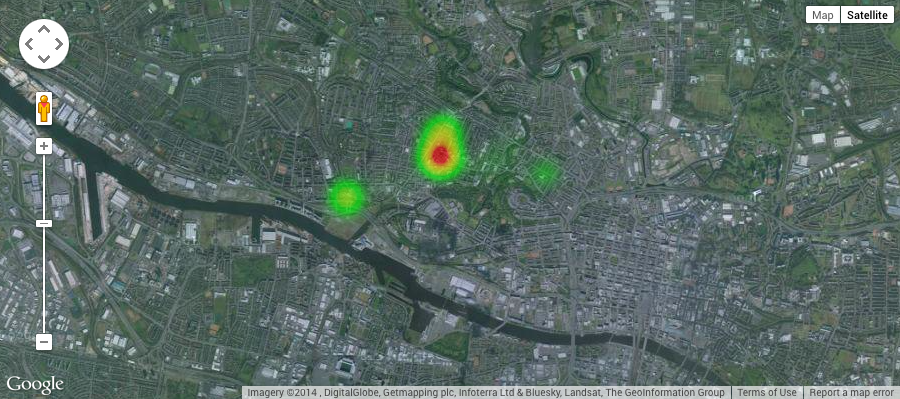
\includegraphics[scale=0.5]{images/screenshots/heatmapscreen.png}
\caption{\textbf{Screenshot showing a Heatmap of the City of Glasgow with data from usage of the Hotsteps pedometer application.}}
\label{impl:heatmapscreen}
\end{figure}

To provide the Heatmaps, I used Google Maps' freely available and usable library. This embeds a number of coordinate points on the map that are colour coded according to the frequency of other data point also plotted nearby. It fits all of the criteria for Heatmaps outlined in the design section, with options to invert the colours for people who suffer from colour blindness. Instead of red amber and green, the data points appear as cooler light blues, dark blues and purples. If the user wants to view less crowded data points, the ability is given 

Heatmaps are maps that have many coordinates placed on them to determine levels of activity visually. Each Heatmap is created by adding all of the coordinates from the query period onto an embeddable Google Map frame defined using Javascript in the website code. As similar to other data displayed, the coordinates are received from a POST request to the appropriate server script, and parsed from the JSON and added to the array of coordinates used by the Heatmap. The coordinates are added as an array of points and entered into the map frame. The areas with the most data points appear as a deep red, areas with less data points as yellow/amber, and the areas with the least data points as a green colour. The less points featured on a specific areas the lighter the colour is. An example of a Heatmap is displayed in Figure \ref{impl:heatmapscreen}. 

One problem encountered with the Heatmap solution used was the appearance of bubbles of activity. Say for example a user had walked down a road and viewed this on a Heatmap on the website. Whilst zoomed out from the ground, the augmented location data would appear as a smooth line of activity, but the closer it was zoomed in the presence of bubbles making up the line would be seen. It is unclear why the Heatmap library is displaying the location data in this way. Checking the database location data shows a constant stream of new coordinates whilst using the app so it cannot be a lack of data. Therefore, it may be that the library tends to clump close data points together, but this is an unproven hypothesis due to lack of development time. It would be important to find out the cause of and fix this issue since a theoretical lack of user enjoyment of the Heatmap feature has consequences for both their usage motivation and a lack of users limits data gathering opportunities.

\subsection{Web Technologies}

The site implementation includes a number of web technologies. PHP is used server side to track user sessions and query the Database in order to be able to create the appropriate cookies for the sites user. The cookies store a number of details about the account that is currently logged in, such as their username and userID both to present to the user and also to be able to seamlessly query the database wilst they use the website to present them with their data.

Javascript is used as the client side language. A great deal of the website functionality is implemented using Javascript. When each page on the website loads, it calls a number of JQuery requests. These JQuery functions send a POST request that will assemble the data that function requires in JSON format. This is then parsed by the Javascript function and displayed by that page in the HTML code.

\subsection{Cookies and Session Handling}

Due to the rejection of using a Web Application Framework (WAF) it was necessary to develop code that would be able to handle a users login across multiple page views, something standard HTTP cannot do. This is achieved through the usage of Cookies set using PHP executed server side as the page loads. When the user logs in, the password given is SHA-256 hashed and the PHP backend performs a query to check that the Username and SHA-256 Hashed Password match that of a registered user. If it does not, they are returned to the Login page and presented with a message saying that their username or password was entered incorrectly. 

If the user did enter an appropriate Username and Password, the PHP backend then queries the Database for the userID corresponding to that user, which is then saved in a Cookie, a small file that resides on the server to keep information between differing HTTP requests the user makes. If the user loads a new page, and that page needs to know the userID, it simply calls and request the value of the Cookie stored on the server.

\subsection{Website Pages}

\subsubsection{Home Page}

The Home Page, defined in \texttt{index.html}, and seen in Figure X.X displays aggregated data about all of the users of the site for that day. At the top Jumbotron, the number of steps made that day, week, month and all time is displayed. The different sections of the page are separated by Bootstrap page headers, which add horizontal lines and Headers to describe the content of that section. This provides a clean website design with different features clearly sepatated over the course of the page. This general design is true for all of the pages on the website. Some pages of interest in the website are described below.

\subsubsection{User Data}

This page allows the user to view their own personal data such inclusing step total.  At the top of the page in a Bootstrap jumbotron is displayed the amount of steps the user has made in that chosen day, 

\subsubsection{Leaderboards}

\begin{figure}[ht!]
\centering
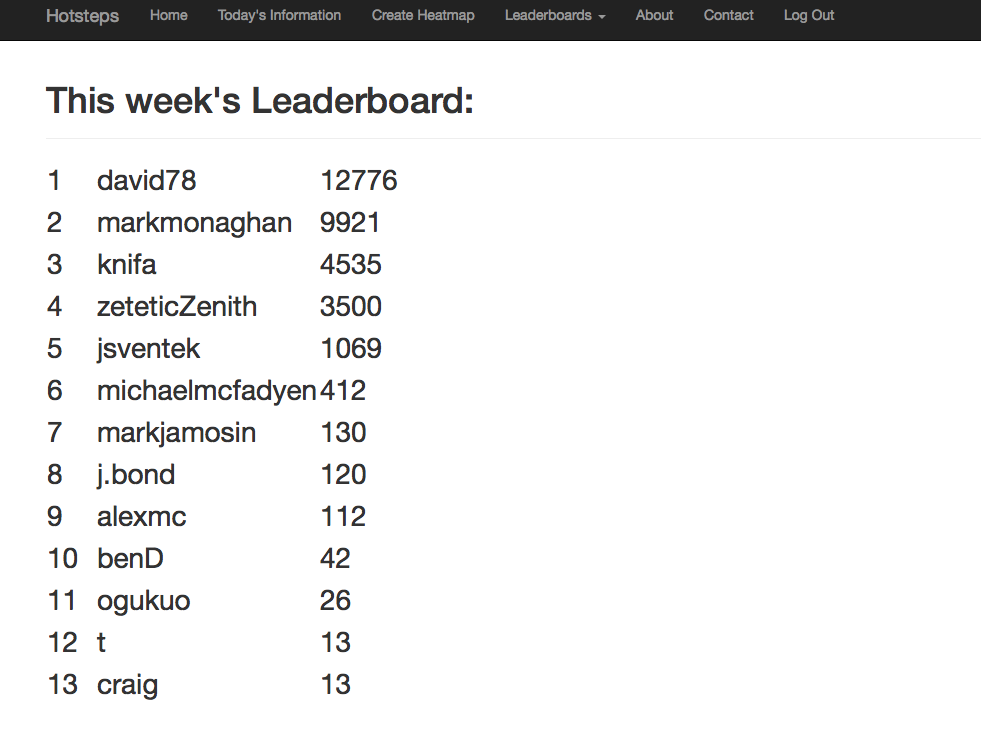
\includegraphics[scale=0.4]{images/screenshots/leaderboardscreen.png}
\caption{\textbf{Screenshot of the weekly leaderboard view of the Hotsteps website, showing the users with the most steps that week ranked in descending order.}}
\label{impl:leaderboardsscreen}
\end{figure}

The three different leaderboards pages enable the user to view Daily, Weekly and Monthly leaderboards of the users with the highest step count displayed in descending order. The leaderboards feature is designed so as to promote competition amongst users of Hotsteps, both increasing the users enjoyment, and also increasing both the quantity and the quality of the data. A screenshot of an example weekly leaderboard is shown in Figure  \ref{impl:leaderboardsscreen}.

\subsubsection{Create Heatmap}

\begin{figure}[ht!]
\centering
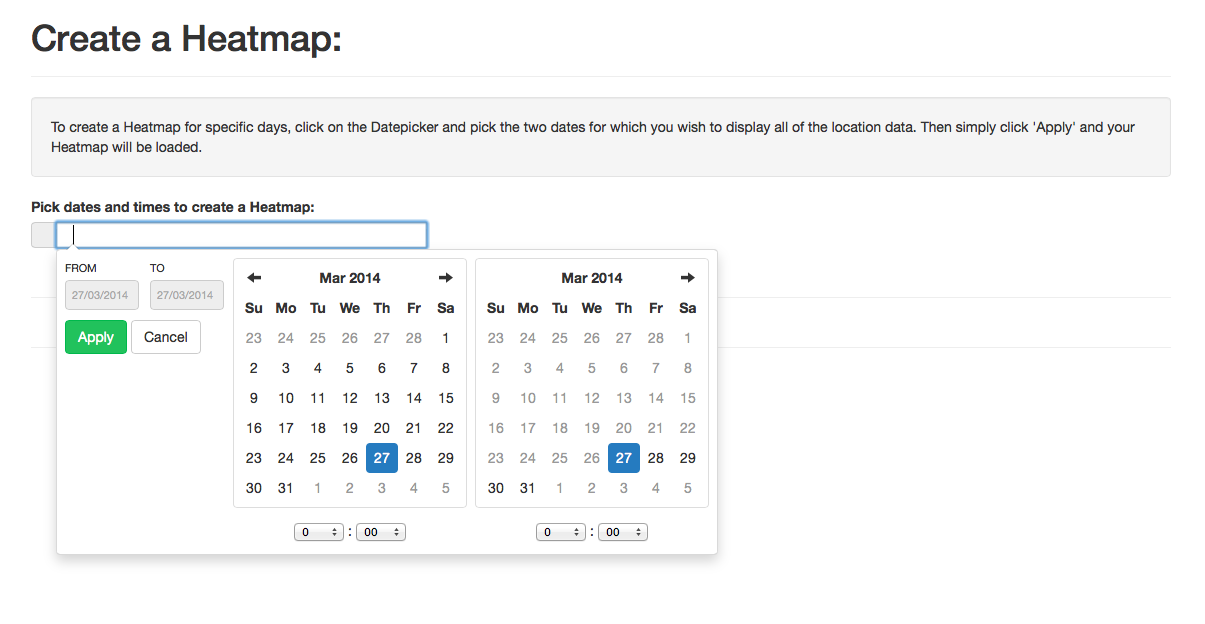
\includegraphics[scale=0.4]{images/screenshots/createheatmapscreen.png}
\caption{\textbf{Screenshot of the User Interface to pick a range of Dates to create a Heatmap from. The date picker used is the Bootstrap styled open-source Date Range Picker for Bootstrap by developer Dan Grossman.}}
\label{impl:createheatmapscreen}
\end{figure}

This function allows the user to pick a range between two dates and view a special heatmap composed of all of the coordinate data from between those date ranges, the UI for which is seen in Figure \ref{impl:createeatmapscreen}. This is possible for both the aggregated and personal data - users who are logged in can click "Create Heatmap" in the "Today's information" view to create a personal one. This feature is designed to appeal to both users of the Hotsteps application as a cool data visualisation feature, and also to prospective users of the data gathered by the Hotsteps application.

\section{Security}

There were many aspects of security thought of when developing the system. In order to be able to use the system, the user must create their own account. This is a necessity due to the storage of user data, but also because of the sensitive location data that is stored amongst users of the application. If it was possible for another user to see a users personal information or location easily, the system would not be secure.

All of the user passwords stored on the system use SHA-256 encyption. As should be obvious, the plain text passwords themselves are never stored. As soon as they are entered, they are ran though the SHA-256 hashing algorithm, and all future references to the password are in that form. SHA-256 encryption is one of the most secure hashing algorithms known, and requires intense processing power to crack for any vaguely uncommon passwords.

Some concerns with security were noted from users of the application. One user noticed that when the user logs into the webpage, that their password is sent via plain-text to the web page that subsequently hashes the given password and checks whether their password is valid for the given user. This is vulnerable to a theoretical man-in-the-middle attack where a user may be packet sniffing data being transported to the server. Due to timescale limitations, it was not possible to fix this given the remaining time, but if development on Hotsteps were to continue, then this should be fixed immediately using the more secure HTTPS instead of standard HTTP. If more users were to discover this, it would undermine confidence in the application, put people off from using the app, lessening the data received.

\section{Version Control}

Throughout development of the project, the Git version control system was used to provide version control for my codebase. This local Git repository was linked to the popular online based repository, Github.  Using GitHub provided numerous benefits to the development process. Firstly, the codebase was backed up remotely and safe in case of a major data-loss. Additionally, Git provides features such as Branching, which enables creation of different branches to aid development. For example, the main branch stores the major revisions that are known to work or at least be stable. If development proceeded on a more challenging aspect of the implementation, then development can be switched onto an 'experimental' branch so as to not endanger the code already in the main branch. Once the work on the experimental branch is complete and tested, this can then be merged back into the master branch.

\section{Problems Faced During Development}

One of the inital problems faced early in development was getting the Server and the Phone to be able to communicate with each other. This was due to network issues. The laptop used for development could create a Wi-Fi hotspot that the phone could access but Android did not recognise such a connection. After some trouble shooting it was discovered that tethering the mobile connection of the phone on the laptop would enable me to access the files located on the Apache server of the computer from the mobile phone using the computers IP address. This enabled development of the Application to be progressed on a local machine until the server was ready to host the files. 

When beginning to develop the application, problems were encountered in trying to understand and instantiate an object of type \texttt{StepCounter} to track the number of steps the user is making. The code as initally received included code to hook into a local database which I would not be using for the purposes of this application, and did not come with clear instructions in regards to implement it. After some trial and error and e-mails to the original author, it was discovered how to instatiate the class by setting a type Boolean \texttt{isSensoring} to be true whilst setting the Pedometer running.

The aforementioned rejection of using a Web Application Framework also caused problems in retrospect. Much time was spent implementing user authentication and session handling code from scratch using PHP and cookies. Usage of a WAF such as Django would have meant that such functionality would have been carried out by the WAF with little additional development time. This time could have been spent implementing more features and bug fixing rather than the many hours that was necessary to implement the user authentication and cookies currently present in the site.

%==============================================================================

\chapter{Testing}

\section{Hotsteps Testing}

One of the challenging aspects of this project was actually testing the application. Pedometers are hard to test in that you need to walk around for large periods of time in a realistic walking environment.

\subsection{Pedometer Testing}

\subsubsection{Step Counting Testing}

The testing of the actual Pedometer of the application is very important, since it was integral for the app to be counting the correct amount of steps. The testing process used a commercial equivalent on the Android platform in order to compare my results. The commercial application that used was Pedometer, as of March 2014 the highest rated Pedometer application on the Google Play Store. Testing involved walking around as usual with both pedometers running. Given that Pedometer is a commercial application, we can make reasonable assumptions about its accuracy but it was also compared with another equivalent application to be sure of its efffectiveness also.

Successive testing sessions on the differences between the Hotsteps application and Pedometer Plus seemsed to confirm around a 500 - 600 difference in step total each day. Pedometer code is notoriously innacurate and hard to test. A number of different factors can affect the accuracy of pedometers.

//INSERT TABLE OF COMPARISONS HERE!

\subsubsection{Battery Life Testing}

In order to test users battery life whilst using the application, I asked users who had had the application for a longer time than the other evaluators their feelings on the battery life used by the application. Most felt fairly satisfied with the battery life, with no one noticing any particular worsening of phone battery life, though in some cases where users had been playing about with the leaderboards and statistics, and continually refreshing, then one user reported it had taken about 20 percent of the battery life in that charge cycle, though on average it seems to settle about 6 percent of battery use when running in the background on a Nexus 4.

\subsubsection{Screen Resolution Issues}

One some devices with a lower screen resolution there may be screen resolution than the phone the app was originally developed for (LG's Nexus 4). issues that occur and have the result of causing UI elements to be cut off. The main area this occurred was the login screen, where on certain devices (Notably the Motorola Moto G and the Samsung Galaxy SIII mini) the 'Create Account' button would not appear fully on screen. Users could generally still press the button (though some users had to be asked to create an account on the website) but this is not a good first impression of the application and the app should be made more robust in handling different screen resolutions. Given the limited time for this project, it was not feasable to handle this given its relatively minor severity, but this would need to be fixed before any larger scale evaluation could take place.

\subsubsection{Found Bugs}

An unsolved bug was uncovered that meant on occasion the application would not function correctly and would crash upon login. This was revealed to be a problem with Location Services, and it has not been uncovered whether it is a bug on the applications code or the API. On all occasions so far, the bug is fixed by having the user turn of and on location functionality on their device and restarting their device. Before a larger scale evaluation was carried out, it would be critical to reveal the cause of and fix this bug as it is fairly severe when it does occur and negaatively impacts people's view of the application.

\subsection{Backend Testing}

It was necessary to test the back end of the application. This was mostly tested though the website and application, and see if the results from querying the database were generally correct. The testing was mostly correct.

\subsection{Website Testing}

In order to test the website, the website was used with a number of different accounts and tested to see if all of the JQuery queries achieved the correct result for that user. A number of bugs were uncovered using this method.

%==============================================================================

\chapter{Evaluation}

\section{User Evaluation}

In order to reach conclusions about the effectiveness of the project, what users liked and disliked about the application it was necessary to carry out a user evaluation. Ideally, given a longer project duration this evaluation would have consisted of a small scale evaluation to get micro-feedback and a larger scale evaluation. The proposed larger scale evaluation would have involved releasing the application on the Google Play Store or similar method of mass software release. Larger data sets would have been achieved and it could have tested how large scale the application could handle.

Given the limited timescales involved, this larger scale evaluation was considered unfeasible, and therefore only the smaller scale evaluation went ahead. In future, a larger scale evaluation would need to take place to harvest data and opinions from a much larger and more representative group of people.

The goals of the evaluation revolved around three aspects. Given that the goal of Hotsteps is to promote an environment where users are motivated to use the application in order to provide the data, there were three aspects that the system has to be successful at to promote future use. These are:

\begin{enumerate}

\item{Is the app interesting enough? If the app is not interesting enough and does not have enough/has the wrong features, then users will not want to use the app in the future. Carrying out the evaluation should establish whether users think the app is interesting enough, and what features could be added to make it more interesting}

\item{Does using the application greatly negatively impact battery life? If the user feels that the app is greatly negatively impacting their battery life, leaving them unable to do what they would like to do with their phone? If this is a very negative impact, users will simply delete the app and therefore limiting the amount of data received.}

\item{Privacy concerns - the app tracks user locations whilst using the app, as well as the number of steps the user takes every 15 minutes. Some users may feel uncomfortable with this, and therefore will not use the app, whilst some users will be OK with this, and as such this would not put them off using the app. The evaluation should discover the range of feelings about this, and hopefully discover strategies that could be used in future versions of the application to mitigate any concerns that may occur.}

\end{enumerate}

\section{Evaluation Strategy}

Upon completion of development of the app and website, it was necessary to carry out a user evaluation to determine from the eyes of end users how well I had achieved what I set out to do and what could be implemented in future from the eyes of the users of the application.

When thinking about participants to use in the evaluation, it was necessary to consider a wide range of users so that the evaluation reflected opinions from a number of different groups of people. There were a number of instant limitations to the group of users that could take part in the user evaluation. The application developed only works on Android devices with Android version 3.0 and above. The limitation was chosen based upon updated UI guidelines and technology introduced with that update. Therefore, the evaluation sample users were fifteen people - five women and ten men, with a variety of age groups ranging from 18 to 53. One concern is the somewhat lower prevalence of women in the sample - future evaluation might wish to have slightly more women than men in order to balance out the results. 

One issue with the evaluation as carried out was that the participants were not being compensated for taking part in the user evaluation, and a worry was that the users would not bother to use the application for any length of time. This could also be seen as a good thing, for, if example, the users did not feel they had to sugar-coat their feelings because they were being recompensated.
 
Due to the theoretical privacy concerns raised by the application, it was necessary to gather user consent from all of my participants. This was carried out in a two stage process - 1) When the user had agreed to be a part of the evaluation, they were made to read and sign a form that explained to them that the application and website would be tracking information about the number of steps they made, and location data about where they used it. It was also explained to them the reasons for carrying out the evaluation, and given my name and contact e-mail address if they wanted to contact me about any concerns or questions that they had. Finally, it was explained to them that they could leave the evaluation at anytime if they felt uncomfortable about the application or the process, and that there would be no embarrassment for doing so.

During the user testing stage, there was regular bug updates and features added to the application in response to user feedback.

The pedometer application developed was then evaluated. The main supervised portion of the evaluation was based upon the website, given that the application was designed to work in the background, without having intensive use by the user.

\section{Evaluation Execution}

The website evaluations took place in a controlled lab environment, on a lab PC running Scientific Linux and the latest version of the open-source Chromium web browser. Participants were asked to download the latest version of the application APK onto their device a day or so before the lab based experiment, and were asked to use the app for a day or so during their day to day business. This fulfilled two functions. It allowed the user to have experience of using the application and help them form their opinions of the app. Additonally, it allowed the user to harvest data before the evaluation began giving the enough data in their account to be able to use all of the features of the website as intended.

When the evaluation began users were asked to fill out a form thanking them for taking part in the evaluation and explaining to the user what would be happening in the evaluation, that think-aloud would be in operation and they could speak their thoughts as they operated the website. They were then given a sheet that included a list of operations that the user might want to try out. This means that the user had an idea of what they could use the website to do but that the evaluation was not as rigid as a standard walkthrough. This gives the user a greater idea of how it would feel in real usage. The user was given as long as they felt that they needed to use the website. This was usually around 5 minutes long for most of the users.

Once the user had completed the website evaluation, they were asked to fill out the questionnaire and then carry out a short interview that lasted about 5 minutes. The interview questions were the same as those asked in the questionnaire, with the questioner usually asking the interview to give reasons as to why they answered that way. This interview was recorded for the purpose of being able to use and build upon the exact information glamed from the earlier questionnair. T By combining both pieces of data, it was possible to get a good viewpoint of how users feel about the app, their likes, dislikes and what they felt could be improved about the system.

Once the evaluation was over each user was thanked for taking part in the evaluation, and asked to email about any questions or concerns they may have. They were also told than once the final project report had been published, participants would have access to the report and read the conclusions if they so desired.

\section{Evaluation Questionnaire}

The questions asked of the users during the evaluation were as follows. Users were asked to circle the number that best fit their view for each of these quesions or statement, with 1 being disagree and 5 being agree:

\begin{enumerate}

\item{Do you enjoy using Hotsteps at its current stage of development?}

\item{Hotsteps would motivate me to walk more in the future.}

\item{Would you like to continue using Hotsteps from now on?}

\item{Did you feel that the Android application was easy to use?}

\item{Did you feel that the Android application needed additional features?}

\item{Did you feel that the website was easy to use?}

\item{Did you feel that the Website needed additional features?}

\item{How concerned are you about privacy issues whilst using Hotsteps?}

\item{Any other thoughts about Hotsteps? What new features would you like, likes/dislikes, privacy concerns?}

\end{enumerate}

\section{Bug fixes to implement after evaluation}

The 'Think-aloud' portion of the evaluation exposed some bugs occurring on other Android devices and the website that would need to be fixed before the subsequent large scale evaluation, as they could negatively impact both peoples perception of and usage levels of the application and system. A major bug uncovered is that sometimes the app crashes upon log-in when the connection to Location Services is being established. Whilst the code should handle failures in establishing connection, on many devices it does not and in any case this bug sometimes occurs when location services is correctly turned on at a device level. More debugging will need to be carried out to determine the cause of this bug. Is it a difficiency in the Hotsteps code, or a problem with the Google Play Services code itself?.

Additionally, the quality of the charts produced on the website was of massively varying qualiy between browsers. Using Firefox, they simply did not load at all, on Safari, Chrome and Chromium the bars of the bar chart loaded but not any scale or labelling. Opera had the best performance with regards to the charts produced by JAwesomeChart, appearing nominally as they should look, though with some squashing on the X-axis. More remedial work will need to be carried out on the website charts, and if fixing these issues looks infeasible, then a move to a different charting library should be considered.

\section{Evaluation Results}

N.B The raw numerical results from the evaluation are given in Appendix A.

\subsubsection{Think Aloud Evaluations}

Some useful unprompted user feedback game from users whilst they were using the website under the principle of "think aloud", where users say what they are thinking of in relation to the evaluation at any time. 

\subsubsection{Question 1}

Do you enjoy using Hotsteps at its current stage of development?
//insert Histogram here

Mean:
Mode: 
Standard Deviation: 

There were a variety of different reasons given for peoples enjoyment of Hotsteps aspart of their usage during the evaluation. 

\subsubsection{Question 2}

//insert Histogram 

Mean:
Mode:
Standard Deviation:

\subsubsection{Question 3}

//insert Histogram here

Mean:
Mode:
Standard Deviation:

P7 responded that they would like to continue using Hotsteps "because it was so simple and easy to set up", and that his "phone was in his pocket anyway". 

\subsubsection{Question 4}

//insert Histogram here

Mean:
Mode:
Standard Deviation:

\subsubsection{Question 5}

//insert Histogram here

Mean:
Mode:
Standard Deviation:

\subsubsection{Question 6}

//insert Histogram here

Mean:
Mode:
Standard Deviation:

\subsubsection{Question 7}

//insert Histogram here

Mean:
Mode:
Standard Deviation:

\subsubsection{Question 8}

//insert Histogram here

Mean: 2.66667
Mode:
Standard Deviation: 1.44749

There were a wide variety of users responses to the privacy concerns of Hotsteps. Four of the partipants described themselves in agreement or strong agreement with the statement in the questionnaire. Six of the participants disagreed with the position, 

%==============================================================================

\chapter{Discussion}

The results of the evaluation suggest that Hotsteps has some merit in doing what it sets out to do, but that it would require a large amount of additional work to live up to users full expectations. Additionally, some users reported a number of privacy concerns about Hotsteps tracking their locations, though these users also helped establish a number of ways that this could be alleviated. Users liked the ideas behind the application, such as the simple setup and tracking, as well as the heatmaps and leaderboards,  but were less optimistic about some of the implementation aspects. For example, users were generally impressed with the large scale nature of the application and liked the usage of the website to view the Heatmaps, but some users also noted a lack of features and some bugs during the evaluation that limited their enjoyment.

\section{Does the app motivate the user to use the app?}

The evaluation showed that the ideas behind the app have merit and users would definitely be interested in using such a system, provided that some of the issues uncovered.

The evaluation showed that users generally enjoyed using the app. Participants were generally most impressed by the Heatmap features, and some noted that the presence of leaderboards would invoke a sense of competion in them, motivating them to coninue using the app in order to try and progress up the rankings.

Some participants noted that in comparison to other tracking applications that require some degree of set-up before a period of activity is started, the Hotsteps tracker was instant and ready to go upon login, tracking and syncing the appropriate data, leaving them free to start walking and being tracked much quicker than other applications they had used. 

Some users felt that the number of features was limited and more social features would be a feature that would motivate them to use Hotsteps. One user, when prompted for additional features they would like, responded with a feature similar to the removed "Goals" feature, with achievements and medals.

Some users noted that since it would not make them walk anymore than it normally would since they tended not to walk so much to begin with. Given the lack of focus on increasing activity in this study, as long as these users were not actively put off using the app then it still provides more data by-products. 

\section{Battery Issues}

Whilst not a formal part of the evaluation process, some users reported back with their feelings on battery life whilst they used the app as part of the evaluation. P6 commented after the interview to the demonstrator that he had been using the application intensively one day, manually syncing andchecking leaderboards frequently throughout the day and the reported battery usage for the Hotsteps app was 20 percent according to the Android OS system level power tracking capabilities.  He noted that this was unlike his usual experience, where Hotsteps had generally required about six percent of power usage on his Nexus 4. One take from this is that the network operations themselves are battery intensive but the mitigation techniques involving only syncing every 10 minutes help maintain battery life. 

\section{Feelings of Users on privacy concerns}

Despite the fact that almost all of users who took part in the evaluation commented on how "cool" the Heatmaps were, The evaluation found mixed feelings on the issue of privacy whilst using Hotsteps as it is currently implemented. The average questionnaire score amongst the users was exactly three, as a result of some people caring greatly, some not caring at all,  and a few users with an in-between question. One user that cared little noted that they "don't care about their locations being tracked", adding that they had "an Android phone, and Google does the same thing anyway". Whilst this is indeed true, users have the option of turning this off, and regardless, it was assumed that Google would be more trusted in storing user data rather than the Hotsteps system. 

The users that noted strong privacy concerns whilst using Hotsteps, were generally concerned about the issues that if they left the app running in their house, then their abode would appear as very red on the Heatmap. These users were uncomfortable with the possibility of this being used in a harmful manner, though  in real usage users are only able to see their own personal locational Heatmaps on their personal page, and it is required to log-in. It was decided to prioritise the views of those that did feel privacy concerns, as those that did not were unlikely to feel disadvantaged if different account level security options were put in place for those users that did indeed have concerns. Afterall, it was important that no user would be actively put off using the app in future due to concerns that can be alleviated.

A number of users offered remedial actions when asked in the interview. One user noted that they were not uncomfortable with their location data being placed on a Heatmap in general, but that they were worried about the possibility of identifying where the user lived. Therefore, given the lack of any inconvenience implementing this would cause, it will be worth making the script that adds location data to the Database to be much more 

Users generally expressed a high degree of concern over the location tracking functionality of the application whilst still liking the feature. The main ethics concern from evaluated users was not necesssarily their movements being tracked on a Heatmap in general, but that in certain circumstances where little usage had occurred it was possible to enter large amounts of data in a specific point such as where they lived, or more obscure places they visited often.

Given the lack of larger scale evaluation, some of the conclusions made in this report would require further investigation on more users before being made final. More data would need to be uncovered about the likelihood of increasing walking activity and usage of the app, but the evaluation carried out could inform the areas of focus in the larger scale evaluation.

\section{Proposed uses for Data}

Whilst it is not the goal of this project to recommend a specific use or uses of the data tat is created and harvested through usage of Hotsteps, there are a number of theoretical areas of interest for what the step totals by time and Heatmap functionality could be used for. One of these is urban planning. Planners could see what areas of the city are busy during given days or given times of day, what parks are most popular amongst users and areas that users generally avoid or has little usage of the app. As an extension to this, consider the possibilty of a person looking to establish a business - this person could look at the information on the site and see what areas have a high foot based traffic, as well as the times of day where those areas are popular.

Tourists may also find such data useful. New vistors to the city could look at the data on the website to find busy areas if they were looking to find some buzz, or if they wanted peace and quiet they could look for areas with less activity.

Whilst not a focus of the application itself for a variety of reasons, there may be some interest in health planning to the information gleamed from the application - it could be seen the areas of the city where walking activity is at its highest, and where it is low, perhaps giving a sign to people to focus efforts of public health programs and activity promotion amongst those areas.

It is important to point out that any such change in the usage of the data produced by Hotsteps would need to be in conjunction with a change to the terms of service of the system, informing what organisations of people could use the data that they have provided to the system, and what that data could be used for.

\section{Future Work}

Given the results of testing the application and carrying out an evaluation has provided a roadmap for the areas that should be focused on in any subsequent development of Hotsteps. In future, there are a number of features that should be implemented, as backed up by my user study. Whilst the application is programmed to be large scale, if the number of users and ferocity of use suddenly became incredibly large then the current set up might not be sufficuent to handle all of the traffic and data that would come along with that. In order to test this, it will be necessary to carry out a larger scale evalutation focussed on mass use of the system simultaneously (look at above 50 simulataneous users to begin with, and slowly scale up the scale of the evaluation whilst the quality of service and use is holding up.

Given that a large percentage of smartphone users use the iOS mobile Operating System, there are a number of prospective users who are simply unable to use the application whilst there is no iOS version of the application. If the app became popular or it was decided that more users were needed, an iOS version could help facilitate this. One thing that it would be necessary to guarantee is that the level of functionality could be guaranteed across any of the platforms that the app runs across - users must be able to have the same accounts between all of the different platforms, and be able to log into the website and see the shared data regardless of what platform it originated on. This would also help the goal of carrying out a larger scale evaluation - the more could be users, the greater the chance of being used at a large scale.

Also following user feedback, t would be good at looking at extending the functionality of the apps themselves - the evaluation suggested that users think that these are fairly bare-bones and lacking in features. The first step in executing this would be to move the functionality of the website to also be available on the applications. Having access to richer data with the website would make the application much more useful than it is currently and stuff.

Further work may also be needed to improve the look and feel of the Heatmaps that are shown in the website. Currently, these appear as clusters of 'blobs' in the map, not as a contiguous line that would be preferred given the data provided to the map. It may be possible to fix this using the current Google provided library, or it may be necessary to look into other libraries available or possibly development of a custom solution to closely adhere to the necessary functions required by the system.

Additionally, the users concerns over privacy would need to be addressed. There are a number of ways that this could be achieved. The algorithm that adds locations to the database could be more aware of repeated input from close locations over the course of the day per user.

%==============================================================================

\chapter{Conclusion}

The application made shows a degree of promise, but will require additional development time and a larger scale evaluation before any final conclusions about its effectiveness in achieving its goals can be made. In the mean time, there are a number of features that can be added based upon user feedback in order to improve usage motivation, and also tackle some of the privacy issues that arised during the user evaluation. Users generally liked and enjoyed the service, and were impressed by the Heatmap functionality on the website, but a number noticed some simple design issues and bugs that affected their enjoyment of the system.

Another issue that could be used . 

\section{Overall success}

Overall, the project was a reasonable success. Whilst at an early stage in research, there was enough user enjoyment of the app as it stands to continue development to at least a stage where a more arduously tested and less buggy version of Hotsteps could be released and evaluated on a larger scale. This would truly test the large scale capabilities and whether users feel the motivation to use the app for a longer period of time than they did during this study. At this stage a further evaluation could be carried out amongst people, or organisations or users who may find that data produced by the apps users interesting, to see if they would have any interesting use for the data, or any other features they feel could be added to the system to increase the usefulness of the data to them.

%==============================================================================

\chapter{Appendix}

\section{Bibliography}

Luis von Ahn and Laura Dabbish. 2004. Labeling images with a computer game. In Proceedings of the SIGCHI Conference on Human Factors in Computing Systems (CHI '04). ACM, New York, NY, USA, 319-326.

Marek Bell, Stuart Reeves, Barry Brown, Scott Sherwood, Donny MacMillan, John Ferguson, and Matthew Chalmers. 2009. EyeSpy: supporting navigation through play. In Proceedings of the SIGCHI Conference on Human Factors in Computing Systems (CHI '09). ACM, New York, NY, USA, 123-132.

Swan, Melanie. "Emerging patient-driven health care models: an examination of health social networks, consumer personalized medicine and quantified self-tracking." International journal of environmental research and public health 6.2 (2009): 492-525.

Li, Ian, Anind Dey, and Jodi Forlizzi. "A stage-based model of personal informatics systems." Proceedings of the SIGCHI Conference on Human Factors in Computing Systems. ACM, 2010.

HERMAWATI, S. and LAWSON, G., 2013. Managing obesity through mobile phone applications: a state of the art review from a user-centred design perspective Personal and Ubiquitous Computing. 2014

A Morrison, O Brown, D McMillan, M Chalmers.Informed Consent and Users' Attitudes to Logging in Large Scale Trials. CHI Extended Abstracts, 1501-1506, 2011.

Krumm, J. A survey of computational location privacy, Personal Ubiquitous Computing, 13(6) 391-399 (2009)


\section{Evaluation Results - Quantitative Data}

\begin{figure}[ht!]
\centering
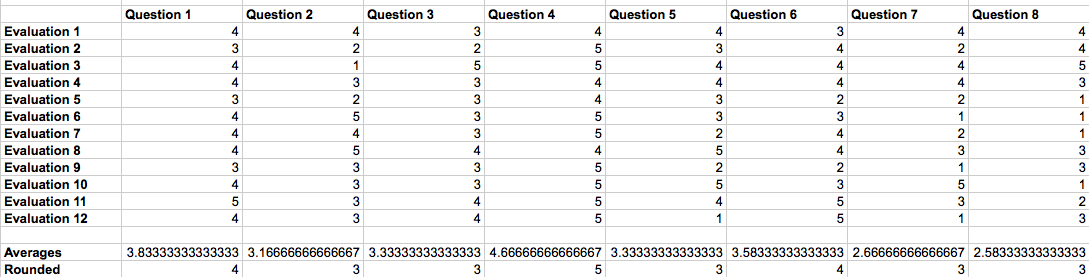
\includegraphics[scale=0.4]{images/screenshots/resultsscreen.png}
\caption{\textbf{Overview of the results of the evaluation and the questions given in Section 7.0.7}}
\label{apndx:resultsscreen}
\end{figure}

\section{Participation Data and Interview Length}

Participant 1: Interview lasted 1:39 
Participant 2: Interview lasted 2:46
Participant 3: Interview lasted 6:01
Participant 4: Interview lasted 3:29
Participant 5: Interview lasted 2:38
Participant 6: Interview lasted 2:57
Participant 7: Interview lasted 2:05
Participant 8: Interview lasted 3:32
Participant 9: Interview lasted 3:28
Participant 10: Interview lasted 2:40
Participant 11: Interview lasted 3:19
Participant 12: Interview lasted 3:04
Participant 13: Interview lasted 4:07
Participant 14: Interview lasted 3:52
Participant 15: Interview lasted 3:20
 
\section{Glossary of common terms and abbreviations used}

Android - An open-source Mobile Operating System with development lead by Google. Currently the most popular Mobile OS, with XX percent of the market as of March 2014. The basis of Android is the Android Open-Source Project, which consists of the Operating System and a limited number of Open-Source applications. On top of AOSP is Google Play services, which provides a number of Google based applications and access to the Google Play Services API.

Google Play Services - An API that enables Android developers to access Google provided services such as Mapping. In the Android application there are regular calls to this API to request the current location.

Tethys - the server located within the school that currently hosts the PHP backend and Database of Hotsteps.

Javascript - Client side language to provide web functionality.

PHP - (A recursive backronym for PHP: Hypertext Preprocessor) is a Server side scripting language, but it can also be used as a general purpose programming language. Handles database querying, cookies and session handling. One of the most common server side languages, installed on the vast majority of the world'sa web servers.

mySQL - An open-source relational Database Management System (DBMS). Very common usage.

HTTP - Hyper Text Transfer Protocol (HTTP) enables clients and servers to talk to each other using structured text to relay information.

POST Request - Information sent via HTTP while requesting a website. More secure than GET requests as the information is not visible as in GET requests.

GET Request - Information sent via HTTP to a server. The information sent is encoded in the URL, meaning it is less ecure than POST requests.

Apache Server - Software to provide server functionality. The server used to provide the website, Database and PHP scripts for the project are hosted on an Apache server.

APACHE License - An open-source licence by the Apache foundation. Software used in this project, such as Android and Apache web server, is released under this license.

Accelerometer - Detects acceleration. Built into every modern smartphone and is used in the Application as part of the step detection.

Gyroscope - Detects movement in space, this is also used to detect the users steps in the Pedometer.

APK - The filetype for Android application files. Consists of the application and a special manifest file. Similar to Java jar files.

\section{URLs to Open-Source technologies used}

Bootstrap: http://bootstrap.com

\end{document}